%===============================================================================
% zentrale Layout-Angaben und Befehle
%===============================================================================
%
\RequirePackage{ifpdf}
\ifpdf
\documentclass[pdftex, a4paper, 12pt]{article}
\else
\documentclass[a4paper, 12pt]{article}
\fi
\usepackage{german}
\usepackage[latin1]{inputenc}
\usepackage{fancyhdr}
\usepackage[T1]{fontenc}
\usepackage{ae}
\usepackage{color}
\usepackage[printonlyused]{acronym}
%
\ifpdf
\usepackage[pdftex,bookmarksopen,bookmarksnumbered]{hyperref}
\usepackage[pdftex]{graphicx}
\pdfcompresslevel=9
\else
\usepackage{url}
\usepackage[dvips]{graphicx}
\fi
%
% ausf�hrlichere Fehlermeldungen
\errorcontextlines=999
%
% Page-Layout
\setlength\headheight{14pt}
\setlength\topmargin{-15,4mm}
\setlength\oddsidemargin{-0,4mm}
\setlength\evensidemargin{-0,4mm}
\setlength\textwidth{160mm}
\setlength\textheight{252mm}
%
% Absatzeinstellungen
\setlength\parindent{0mm}
\setlength\parskip{2ex}
%
% Anweisung zur Erstellung der Titelseite
% #1 = Name des Seminars
% #2 = Name der Ausarbeitung
% #3 = Autor
% #4 = Betreuer
% #5 = Semester, z.B. SoSe 2002
% #6 = {Bachelor|Master|Diplom}
\renewcommand{\maketitle}[6] {
\pagenumbering{Alph}
  \begin{titlepage}
  \centering
    \begin{minipage}[t]{16cm}
      \begin{minipage}{3cm}
        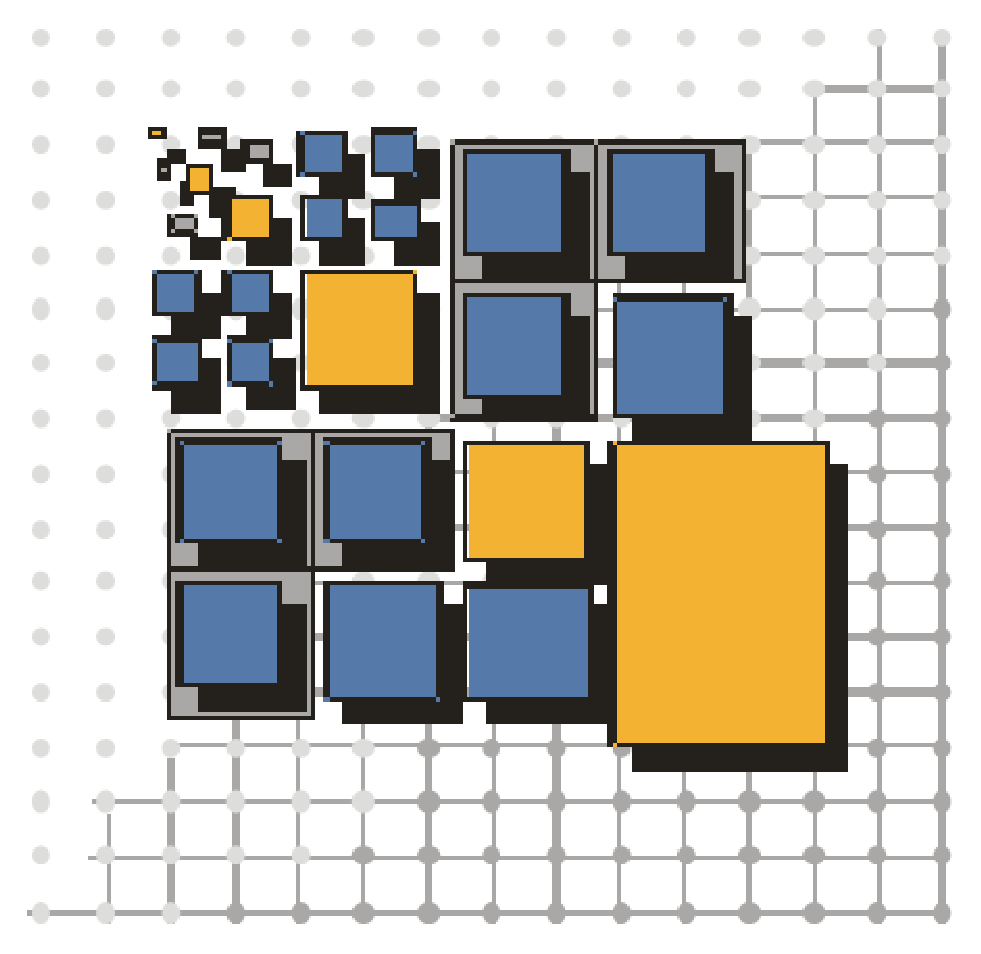
\includegraphics[height=26mm]{include/logo}
      \end{minipage}
      \hfill
      \begin{minipage}{9cm}
        \centering
        Otto-Friedrich-Universit�t Bamberg\\[12pt]
        {\Large Lehrstuhl f�r Praktische Informatik}
      \end{minipage}
      \hfill
      \begin{minipage}{3cm}
        
\includegraphics[height=26mm]{include/UB-Logo-neu_blau-cmyk}
      \end{minipage}
    \end{minipage}\\[108pt]
    {\LARGE Ausarbeitung}\\[18pt]
    Im Rahmen des #6-Seminars\\[12pt]
    {\Large\bf #1}\\[92pt]
    Zum Thema:\\[24pt]
    {\Huge #2}\\
    \vfill
    \begin{minipage}{\textwidth}
      \center
      Vorgelegt von:\\
      {\Large #3\\[18pt]}
      Betreuer: #4\\[12pt]
      Bamberg, #5
    \end{minipage}
  \end{titlepage}
}
%
% setzen nur von fusszeile
\newcommand{\setbottom}
{
\pagestyle{fancy}
\fancyhf{}
\fancyfoot[LO]{\footnotesize\sc Lehrstuhl f�r Praktische Informatik}
\fancyfoot[RO]{\thepage}
\renewcommand{\headrulewidth}{0pt}
\renewcommand{\footrulewidth}{0pt}
}
%
% Einbindung eines Bildes
% #1 = label f�r \ref-Verweise
% #2 = Name des Bildes ohne Endung relativ zu images-Verzeichnis
% #3 = Beschriftung
% #4 = Breite des Bildes im Dokument in cm
\newcommand{\bild}[4]{%
  \begin{figure}[htb]%
    \begin{center}%
      \includegraphics[width=#4cm]{images/#2}%
      \vskip -0.3cm%
      \caption{#3}%
      \vskip -0,2cm%
      \label{#1}%
    \end{center}%
  \end{figure}%
}
%
% Umgebung f�r Fliesstext um Grafik
% #1 = Ausrichtung: r, l, i, ...
% #2 = Breite des Bildes in cm
% #3 = Name des Bildes ohne Endung relativ zu images-Verzeichnis
% #4 = Beschriftung
% #5 = label f�r \ref-Verweise
\newcommand{\fliesstext}[5]{%
\begin{wrapfigure}{#1}{#2cm}%
\includegraphics[width=#2cm]{images/#3}%
\caption{#4}%
\label{#5}%
\end{wrapfigure}%
}
%